% CS631D Advanced Programming in the UNIX Environment
% Author: Jan Schaumann <jschauma@netmeister.org>
% $Id: slides.tex,v 1.4 2004/08/01 03:23:37 jschauma Exp $
\special{! TeXDict begin /landplus90{true}store end }

\documentclass[xga]{xdvislides}
\usepackage[landscape]{geometry}
\usepackage{graphics}
\usepackage{graphicx}
\usepackage{colordvi}
\usepackage[normalem]{ulem}

\begin{document}
\setfontphv

%%% Headers and footers
\lhead{\slidetitle}
\chead{CS631 - Advanced Programming in the UNIX Environment}
\rhead{Slide \thepage}
\lfoot{\Gray{Lecture 04: File Systems, System Data Files, Time \& Date}}
\cfoot{\relax}
\rfoot{\Gray{\today}}

\vspace*{\fill}
\begin{center}
	\Hugesize
		CS631 - Advanced Programming in the UNIX Environment\\
		-- \\
		File Systems, System Data Files, Time \& Date
	\hspace*{5mm}\blueline\\ [1em]
	\Normalsize
		Department of Computer Science\\
		Stevens Institute of Technology\\
		Jan Schaumann\\
		\verb+jschauma@stevens.edu+\\
		\verb+https://stevens.netmeister.org/631/+
\end{center}
\vspace*{\fill}

\subsection{HW\#1 Notes: Avoid useless comments}
\begin{verbatim}
/* open the source file */
if((fd_src = open(argv[1],O_RDONLY)) == -1){

//check the number of commandline argument
if(argc != 3)

//output the usage of this app.^M
if(argc != 3){^M
        (void)fprintf(stderr,^M
                "Usage: %s [file1] [file2]\n\^M


/* Buffer size */
#define BUFSIZE 4096

/* Check if the destination is a directory */
if(stat(argv[2], &s) != -1 && S_ISDIR(s.st_mode))
\end{verbatim}
\Normalsize

\subsection{HW\#1 Notes}
Errors go to \verb+stderr+, please!  Use
\verb+strerror(3)+/\verb+perror(3)+. \\

\begin{verbatim}
printf("malloc failed\n");

printf("Cannot read your source file.\n");


  if(!S_ISREG(src.st_mode) )
  {
    printf("Source file is not a regular file\n");^M



            printf("Unable to read %s\n",input_src
                   );

\end{verbatim}

\subsection{HW\#1 Notes: Check all return codes!}
\begin{verbatim}
file_in_dir = calloc(len, 1);
snprintf(file_in_dir, len, "%s/%s", argv[2], basename);

int isDirectory(char* testString) {^M
        struct stat dir;^M
        if(stat(testString, &dir) >= 0) {^M
                if(S_ISDIR(dir.st_mode))^M
                        return 1;^M
        }^M
        return 0;^M
}^M

dstPath = (char*)malloc(strlen(argv[2]) + strlen(filename) + 2);
dstPath = strcpy(dstPath, argv[2]);

dir_fd=dirfd(dir);
dest_file=openat(dir_fd,argv[1],O_WRONLY | O_CREAT , 0641);
\end{verbatim}
\Normalsize

\subsection{HW\#1 Notes: Don't overflow your buffers!}
Use of \verb+strcat(3)+ etc. considered harmful.
Use \verb+strlcat(3)+/\verb+strlcpy(3)+ etc. instead.
Know your buffer boundaries!
\begin{verbatim}
char *writePath = argv[2]
bname = basename(readPath);
strcat(writePath,"/");
strcat(writePath,bname);

char filename[100] = "";
strcat(filename, argv[2]);
strcat(filename, "/");
strcat(filename, getFilename(argv[1]));

target_path = (char *)malloc(sizeof(argv[2]) + 2 +
      sizeof(basename(argv[1])));
(void)strcat(target_path, basename(argv[1]));
\end{verbatim}
\vspace{.15in}
But beware: \verb+sizeof != strlen(3)+ See: \verb+sizeof.c+
\vspace*{\fill}

\subsection{HW\#1 Notes: Goldilocks Whitespace}
\begin{verbatim}
if((sourceFile=(char*)calloc(strlen(argv[1])+1,sizeof(char)))!=NULL)^M
  strcpy(sourceFile,argv[1]);^M
\end{verbatim}
\begin{center}
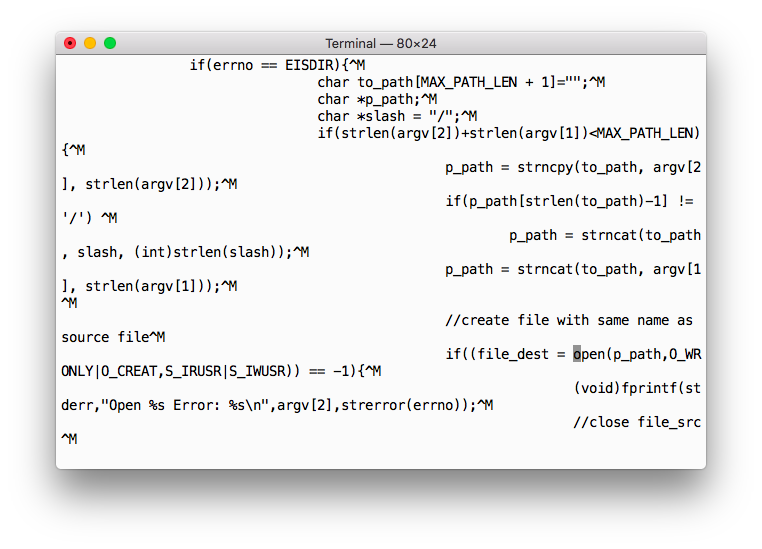
\includegraphics[scale=0.5]{pics/whitespace.eps}
\end{center}

\subsection{HW\#1 Notes: Flow}
\begin{tabular}{l | l}
\begin{minipage}{4in}
\begin{verbatim}

if (condition) {
        some
        long
        block
        here
        with
        if (condition) {
                nested
        } else {
                conditions
        }
} else {
        error
}
\end{verbatim}
\end{minipage} & \begin{minipage}{4in}
\begin{verbatim}

    if (!condition) {
            error
    }

    some
    long
    block
    here
    with
    if (condition) {
            nested
    } else {
            conditions
    }
\end{verbatim}
\end{minipage}
\end{tabular}

\pagebreak

\vspace*{\fill}
\begin{center}
  \Hugesize
	File Systems
	\hspace*{5mm}\blueline\\ [1em]
	System Data Files, Time \& Date
  \Normalsize
\end{center}
\vspace*{\fill}



\subsection{File Systems}
\begin{itemize}
	\item a disk can be divided into logical {\em partitions}
\end{itemize}
\includegraphics[angle=-90,scale=0.9]{pics/fs1.eps}


\subsection{File Systems}
\begin{itemize}
	\item a disk can be divided into logical {\em partitions}
	\item each logical {\em partition} may be further divided into
		{\em file systems} containing {\em cylinder groups}
\end{itemize}
\includegraphics[angle=-90,scale=0.9]{pics/fs2.eps}

\subsection{File Systems}
\begin{itemize}
	\item a disk can be divided into logical {\em partitions}
	\item each logical {\em partition} may be further divided into
		{\em file systems} containing {\em cylinder groups}
	\item each {\em cylinder group} contains a list of {\em inodes} ({\em i-list})
		as well as the actual {\em directory-} and {\em data blocks}
\end{itemize}
\includegraphics[angle=-90,scale=0.9]{pics/fs3.eps}

\subsection{File Systems}
\begin{itemize}
	\item a disk can be divided into logical {\em partitions}
	\item each logical {\em partition} may be further divided into
		{\em file systems} containing {\em cylinder groups}
	\item each {\em cylinder group} contains a list of {\em inodes} ({\em i-list})
		as well as the actual {\em directory-} and {\em data blocks}
\end{itemize}
\includegraphics[angle=-90,scale=0.9]{pics/fs4.eps}

\subsection{File Systems}
\begin{itemize}
	\item a disk can be divided into logical {\em partitions}
	\item each logical {\em partition} may be further divided into
		{\em file systems} containing {\em cylinder groups}
	\item each {\em cylinder group} contains a list of {\em inodes} ({\em i-list})
		as well as the actual {\em directory-} and {\em data blocks}
\end{itemize}
\includegraphics[angle=-90,scale=0.7]{pics/links1.eps}

\subsection{File Systems}
\begin{itemize}
	\item a disk can be divided into logical {\em partitions}
	\item each logical {\em partition} may be further divided into
		{\em file systems} containing {\em cylinder groups}
	\item each {\em cylinder group} contains a list of {\em inodes} ({\em i-list})
		as well as the actual {\em directory-} and {\em data blocks}
	\item a directory entry is really just a {\em hard link} mapping a
		``filename'' to an inode
\end{itemize}
\includegraphics[angle=-90,scale=0.7]{pics/links2.eps}

\subsection{File Systems}
\begin{itemize}
	\item a disk can be divided into logical {\em partitions}
	\item each logical {\em partition} may be further divided into
		{\em file systems} containing {\em cylinder groups}
	\item each {\em cylinder group} contains a list of {\em inodes} ({\em i-list})
		as well as the actual {\em directory-} and {\em data blocks}
	\item a directory entry is really just a {\em hard link} mapping a
		``filename'' to an inode
	\item you can have many such mappings to the same file
\end{itemize}
\includegraphics[angle=-90,scale=0.7]{pics/links3.eps}

\subsection{Directories}
\begin{itemize}
	\item directories are special "files" containing hardlinks
\end{itemize}
\includegraphics[angle=-90]{pics/subdirs1.eps}

\subsection{Directories}
\begin{itemize}
	\item directories are special "files" containing hardlinks
	\item each directory contains at least two entries:
		\begin{itemize}
			\item {\tt .} ({\em this} directory)
			\item {\tt ..} (the parent directory)
		\end{itemize}
\end{itemize}
\includegraphics[angle=-90]{pics/subdirs2.eps}

\subsection{Directories}
\begin{itemize}
	\item directories are special "files" containing hardlinks
	\item each directory contains at least two entries:
		\begin{itemize}
			\item {\tt .} ({\em this} directory)
			\item {\tt ..} (the parent directory)
		\end{itemize}
	\item the link count ({\tt st\_nlink}) of a directory is at least $2$
\end{itemize}
\includegraphics[angle=-90,scale=0.7]{pics/subdirs3.eps}

\subsection{Inodes}
\begin{itemize}
	\item the {\em inode} contains most of the information found in the {\tt stat}
		structure.
\end{itemize}

\subsection{Inodes}
\begin{itemize}
	\item the {\em inode} contains most of the information found in the {\tt stat}
		structure.
	\item every {\em inode} has a {\em link count} ({\tt st\_nlink}):  it
		shows how many ``things'' point to this inode.  Only if this
		{\em link count} is 0 (and no process has the file open) are the
		{\em data blocks} freed.
\end{itemize}

\subsection{Inodes}
\begin{itemize}
	\item the {\em inode} contains most of the information found in the {\tt stat}
		structure.
	\item every {\em inode} has a {\em link count} ({\tt st\_nlink}):  it
		shows how many ``things'' point to this inode.  Only if this
		{\em link count} is 0 (and no process has the file open) are the
		{\em data blocks} freed.
	\item {\em inode} number in a directory entry must point to an {\em inode}
		on the same file system (no hardlinks across filesystems)
\end{itemize}
\includegraphics[angle=-90,scale=0.9]{pics/fs4.eps}


\subsection{Inodes}
\begin{itemize}
	\item the {\em inode} contains most of the information found in the {\tt stat}
		structure.
	\item every {\em inode} has a {\em link count} ({\tt st\_nlink}):  it
		shows how many ``things'' point to this inode.  Only if this
		{\em link count} is 0 (and no process has the file open) are the
		{\em data blocks} freed.
	\item {\em inode} number in a directory entry must point to an {\em inode}
		on the same file system (no hardlinks across filesystems)
	\item to move a file within a single filesystem, we can just "move" the
		directory entry (actually done by creating a new entry, and deleting
		the old one).
\end{itemize}
\includegraphics[angle=-90,scale=0.67]{pics/links2.eps}

\subsection{Inodes}
\begin{itemize}
	\item the {\em inode} contains most of the information found in the {\tt stat}
		structure.
	\item every {\em inode} has a {\em link count} ({\tt st\_nlink}):  it
		shows how many ``things'' point to this inode.  Only if this
		{\em link count} is 0 (and no process has the file open) are the
		{\em data blocks} freed.
	\item {\em inode} number in a directory entry must point to an {\em inode}
		on the same file system (no hardlinks across filesystems)
	\item to move a file within a single filesystem, we can just "move" the
		directory entry (actually done by creating a new entry, and deleting
		the old one).
\end{itemize}
\includegraphics[angle=-90,scale=0.67]{pics/links3.eps}

\subsection{Inodes}
\begin{itemize}
	\item the {\em inode} contains most of the information found in the {\tt stat}
		structure.
	\item every {\em inode} has a {\em link count} ({\tt st\_nlink}):  it
		shows how many ``things'' point to this inode.  Only if this
		{\em link count} is 0 (and no process has the file open) are the
		{\em data blocks} freed.
	\item {\em inode} number in a directory entry must point to an {\em inode}
		on the same file system (no hardlinks across filesystems)
	\item to move a file within a single filesystem, we can just "move" the
		directory entry (actually done by creating a new entry, and deleting
		the old one).
\end{itemize}
\includegraphics[angle=-90,scale=0.67]{pics/links4.eps}



\subsection{{\tt link(2)}}
\small
\setlength{\unitlength}{1mm}
\begin{center}
	\begin{picture}(150,25)
		\thinlines
		\put(0,0){\framebox(130,25){}}
		\put(10,20){{\tt \#include <unistd.h>}}
		\put(10,12){{\tt int link(const char *{\em name1}, const char *{\em name2});}}
		\put(85,3){Returns: 0 if OK, -1 on error}
	\end{picture}
\end{center}
\Normalsize
\begin{itemize}
	\item Creates a link to an existing file (hard link).
	\item POSIX.1 allows links to cross filesystems, most implementations (SVR4, BSD) don't.
	\item only uid(0) can create links to directories (loops in filesystem are bad)
\end{itemize}

\subsection{{\tt link(2)} and {\tt unlink(2)}}
\small
\setlength{\unitlength}{1mm}
\begin{center}
	\begin{picture}(150,25)
		\thinlines
		\put(0,0){\framebox(130,25){}}
		\put(10,20){{\tt \#include <unistd.h>}}
		\put(10,12){{\tt int link(const char *{\em name1}, const char *{\em name2});}}
		\put(85,3){Returns: 0 if OK, -1 on error}
	\end{picture}
\end{center}
\Normalsize
\begin{itemize}
	\item Creates a link to an existing file (hard link).
	\item POSIX.1 allows links to cross filesystems, most implementations (SVR4, BSD) don't.
	\item only uid(0) can create links to directories (loops in filesystem are bad)
\end{itemize}
\vspace{.25in}
\small
\setlength{\unitlength}{1mm}
\begin{center}
	\begin{picture}(150,25)
		\thinlines
		\put(0,0){\framebox(130,25){}}
		\put(10,20){{\tt \#include <unistd.h>}}
		\put(10,12){{\tt int unlink(const char *{\em path});}}
		\put(85,3){Returns: 0 if OK, -1 on error}
	\end{picture}
\end{center}
\Normalsize
\begin{itemize}
	\item removes directory entry and decrements link count of file
	\item if file link count == 0, free data blocks associated with file
		(...unless processes have the file open)
\end{itemize}

\subsection{{\tt link(2)} and {\tt unlink(2)}}
\begin{verbatim}
$ cc -Wall wait-unlink.c
$ ./a.out
$ df .
\end{verbatim}


\subsection{{\tt rename(2)}}
\small
\setlength{\unitlength}{1mm}
\begin{center}
	\begin{picture}(150,25)
		\thinlines
		\put(0,0){\framebox(130,25){}}
		\put(10,20){{\tt \#include <stdio.h>}}
		\put(10,12){{\tt int rename(const char *{\em from}, const char *{\em to});}}
		\put(85,3){Returns: 0 if OK, -1 on error}
	\end{picture}
\end{center}
\Normalsize

If {\em oldname} refers to a file:
\begin{itemize}
	\item if {\em newname} exists and it is not a directory, it's removed
		and {\em oldname} is renamed {\em newname}
\end{itemize}

\subsection{{\tt rename(2)}}
\small
\setlength{\unitlength}{1mm}
\begin{center}
	\begin{picture}(150,25)
		\thinlines
		\put(0,0){\framebox(130,25){}}
		\put(10,20){{\tt \#include <stdio.h>}}
		\put(10,12){{\tt int rename(const char *{\em from}, const char *{\em to});}}
		\put(85,3){Returns: 0 if OK, -1 on error}
	\end{picture}
\end{center}
\Normalsize

If {\em oldname} refers to a file:
\begin{itemize}
	\item if {\em newname} exists and it is not a directory, it's removed
		and {\em oldname} is renamed {\em newname}
	\item if {\em newname} exists and it is a directory, an error results
\end{itemize}

\subsection{{\tt rename(2)}}
\small
\setlength{\unitlength}{1mm}
\begin{center}
	\begin{picture}(150,25)
		\thinlines
		\put(0,0){\framebox(130,25){}}
		\put(10,20){{\tt \#include <stdio.h>}}
		\put(10,12){{\tt int rename(const char *{\em from}, const char *{\em to});}}
		\put(85,3){Returns: 0 if OK, -1 on error}
	\end{picture}
\end{center}
\Normalsize

If {\em oldname} refers to a file:
\begin{itemize}
	\item if {\em newname} exists and it is not a directory, it's removed
		and {\em oldname} is renamed {\em newname}
	\item if {\em newname} exists and it is a directory, an error results
	\item must have w+x perms for the directories containing {\em old}/{\em newname}
\end{itemize}

\subsection{{\tt rename(2)}}
\small
\setlength{\unitlength}{1mm}
\begin{center}
	\begin{picture}(150,25)
		\thinlines
		\put(0,0){\framebox(130,25){}}
		\put(10,20){{\tt \#include <stdio.h>}}
		\put(10,12){{\tt int rename(const char *{\em from}, const char *{\em to});}}
		\put(85,3){Returns: 0 if OK, -1 on error}
	\end{picture}
\end{center}
\Normalsize

If {\em oldname} refers to a file:
\begin{itemize}
	\item if {\em newname} exists and it is not a directory, it's removed
		and {\em oldname} is renamed {\em newname}
	\item if {\em newname} exists and it is a directory, an error results
	\item must have w+x perms for the directories containing {\em old}/{\em newname}
\end{itemize}

If {\em oldname} refers to a directory:
\begin{itemize}
	\item if {\em newname} exists and is an empty directory (contains only .
		and ..), it is removed; {\em oldname} is renamed {\em newname}
\end{itemize}

\subsection{{\tt rename(2)}}
\small
\setlength{\unitlength}{1mm}
\begin{center}
	\begin{picture}(150,25)
		\thinlines
		\put(0,0){\framebox(130,25){}}
		\put(10,20){{\tt \#include <stdio.h>}}
		\put(10,12){{\tt int rename(const char *{\em from}, const char *{\em to});}}
		\put(85,3){Returns: 0 if OK, -1 on error}
	\end{picture}
\end{center}
\Normalsize

If {\em oldname} refers to a file:
\begin{itemize}
	\item if {\em newname} exists and it is not a directory, it's removed
		and {\em oldname} is renamed {\em newname}
	\item if {\em newname} exists and it is a directory, an error results
	\item must have w+x perms for the directories containing {\em old}/{\em newname}
\end{itemize}

If {\em oldname} refers to a directory:
\begin{itemize}
	\item if {\em newname} exists and is an empty directory (contains only .
		and ..), it is removed; {\em oldname} is renamed {\em newname}
    \item if {\em newname} exists and is a file, an error results
\end{itemize}

\subsection{{\tt rename(2)}}
\small
\setlength{\unitlength}{1mm}
\begin{center}
	\begin{picture}(150,25)
		\thinlines
		\put(0,0){\framebox(130,25){}}
		\put(10,20){{\tt \#include <stdio.h>}}
		\put(10,12){{\tt int rename(const char *{\em from}, const char *{\em to});}}
		\put(85,3){Returns: 0 if OK, -1 on error}
	\end{picture}
\end{center}
\Normalsize

If {\em oldname} refers to a file:
\begin{itemize}
	\item if {\em newname} exists and it is not a directory, it's removed
		and {\em oldname} is renamed {\em newname}
	\item if {\em newname} exists and it is a directory, an error results
	\item must have w+x perms for the directories containing {\em old}/{\em newname}
\end{itemize}

If {\em oldname} refers to a directory:
\begin{itemize}
	\item if {\em newname} exists and is an empty directory (contains only .
		and ..), it is removed; {\em oldname} is renamed {\em newname}
    \item if {\em newname} exists and is a file, an error results
	\item if {\em oldname} is a prefix of {\em newname} an error results
\end{itemize}

\subsection{{\tt rename(2)}}
\small
\setlength{\unitlength}{1mm}
\begin{center}
	\begin{picture}(150,25)
		\thinlines
		\put(0,0){\framebox(130,25){}}
		\put(10,20){{\tt \#include <stdio.h>}}
		\put(10,12){{\tt int rename(const char *{\em from}, const char *{\em to});}}
		\put(85,3){Returns: 0 if OK, -1 on error}
	\end{picture}
\end{center}
\Normalsize

If {\em oldname} refers to a file:
\begin{itemize}
	\item if {\em newname} exists and it is not a directory, it's removed
		and {\em oldname} is renamed {\em newname}
	\item if {\em newname} exists and it is a directory, an error results
	\item must have w+x perms for the directories containing {\em old}/{\em newname}
\end{itemize}

If {\em oldname} refers to a directory:
\begin{itemize}
	\item if {\em newname} exists and is an empty directory (contains only .
		and ..), it is removed; {\em oldname} is renamed {\em newname}
    \item if {\em newname} exists and is a file, an error results
	\item if {\em oldname} is a prefix of {\em newname} an error results
	\item must have w+x perms for the directories containing {\em old}/{\em newname}
\end{itemize}

\subsection{Symbolic Links}
\small
\setlength{\unitlength}{1mm}
\begin{center}
	\begin{picture}(150,25)
		\thinlines
		\put(0,0){\framebox(130,25){}}
		\put(10,20){{\tt \#include <unistd.h>}}
		\put(10,12){{\tt int symlink(const char *{\em name1}, const char *{\em name2});}}
		\put(85,3){Returns: 0 if OK, -1 on error}
	\end{picture}
\end{center}
\Normalsize

\begin{itemize}
	\item file whose "data" is a path to another file
	\item anyone can create symlinks to directories or files
	\item certain functions dereference the link, others operate on the link
\end{itemize}
\vspace{.5in}
How do we get the contents of a symlink? {\tt open(2)} and {\tt read(2)}?

\subsection{Symbolic Links}
\small
\setlength{\unitlength}{1mm}
\begin{center}
	\begin{picture}(150,25)
		\thinlines
		\put(0,0){\framebox(130,25){}}
		\put(10,20){{\tt \#include <unistd.h>}}
		\put(10,12){{\tt int symlink(const char *{\em name1}, const char *{\em name2});}}
		\put(85,3){Returns: 0 if OK, -1 on error}
	\end{picture}
\end{center}
\Normalsize

\begin{itemize}
	\item file whose "data" is a path to another file
	\item anyone can create symlinks to directories or files
	\item certain functions dereference the link, others operate on the link
\end{itemize}
\vspace{.5in}
\small
\setlength{\unitlength}{1mm}
\begin{center}
	\begin{picture}(150,25)
		\thinlines
		\put(0,0){\framebox(130,25){}}
		\put(10,20){{\tt \#include <unistd.h>}}
		\put(10,12){{\tt int readlink(const char *{\em path}, char *{\em buf}, size\_t {\em bufsize});}}
		\put(33,3){Returns: number of bytes placed into buffer if OK, -1 on error}
	\end{picture}
\end{center}
\Normalsize
This function combines the actions of {\tt open}, {\tt read}, and {\tt close}. \\
Note: {\em buf} is {\bf not} NUL terminated.

\subsection{File Times}
\small
\setlength{\unitlength}{1mm}
\begin{center}
	\begin{picture}(150,30)
		\thinlines
		\put(0,0){\framebox(130,30){}}
		\put(10,25){{\tt \#include <sys/types.h>}}
		\put(10,16){{\tt int utimes(const char *{\em path}, const struct timeval times[2]);}}
		\put(10,12){{\tt int lutimes(const char *{\em path}, const struct timeval times[2]);}}
		\put(10,8){{\tt int futimes(int {\em fd}, const struct timeval times[2]);}}
		\put(85,3){Returns: 0 if OK, -1 on error}
	\end{picture}
\end{center}
\Normalsize

If {\em times} is NULL, access time and modification time are set to the
current time (must be owner of file or have write permission). If {\em times}
is non-NULL, then times are set according to the {\tt timeval struct} array. For
this, you must be the owner of the file (write permission not enough).  \\

Note that {\tt st\_ctime} is set to the current time in both cases. \\

For the effect of various functions on the access, modification and
changes-status times see Stevens, p. 117. \\

Note: some systems implement {\tt lutimes(3)} (library call) via {\tt
utimes(2)} syscalls.

\subsection{{\tt mkdir(2)} and {\tt rmdir(2)}}
\small
\setlength{\unitlength}{1mm}
\begin{center}
	\begin{picture}(150,30)
		\thinlines
		\put(0,0){\framebox(130,30){}}
		\put(10,25){{\tt \#include <sys/types.h>}}
		\put(10,20){{\tt \#include <sys/stat.h>}}
		\put(10,12){{\tt int mkdir(const char *{\em path}, mode\_t {\em mode});}}
		\put(85,3){Returns: 0 if OK, -1 on error}
	\end{picture}
\end{center}
\Normalsize
Creates a new, empty (except for . and .. entries) directory.  Access
permissions specified by {\em mode} and restricted by the {\tt umask(2)} of
the calling process.
\vspace{.5in}
\small
\setlength{\unitlength}{1mm}
\begin{center}
	\begin{picture}(150,25)
		\thinlines
		\put(0,0){\framebox(130,25){}}
		\put(10,20){{\tt \#include <unistd.h>}}
		\put(10,12){{\tt int rmdir(const char *{\em path});}}
		\put(85,3){Returns: 0 if OK, -1 on error}
	\end{picture}
\end{center}
\Normalsize

If the link count is 0 (after this call), and no other process has the directory open, directory
is removed. Directory must be empty (only . and .. remaining)

\subsection{Reading Directories}
\small
\setlength{\unitlength}{1mm}
\begin{center}
	\begin{picture}(150,55)
		\thinlines
		\put(0,0){\framebox(130,55){}}
		\put(10,50){{\tt \#include <sys/types.h>}}
		\put(10,45){{\tt \#include <dirent.h>}}
		\put(10,37){{\tt DIR *opendir(const char *{\em filename});}}
		\put(70,32){Returns: pointer if OK, {\tt NULL} on error}
		\put(10,25){{\tt struct dirent *readdir(DIR *{\em dp});}}
		\put(45,20){Returns: pointer if OK, {\tt NULL} at end of dir or on error}
		\put(10,13){{\tt void rewinddir(DIR *{\em dp});}}
		\put(10,8){{\tt int closedir(DIR *{\em dp});}}
		\put(85,3){Returns: 0 if OK, -1 on error}
	\end{picture}
\end{center}
\Normalsize

\begin{itemize}
	\item read by anyone with read permission on the directory
	\item format of directory is implementation dependent (always use readdir and
		friends)
\end{itemize}
\vspace{.25in}

{\tt opendir}, {\tt readdir} and {\tt closedir} should be familiar from our
small {\tt ls} clone.  {\tt rewinddir} resets an open directory to the
beginning so readdir will again return the first entry. \\

For directory traversal, consider {\tt fts(3)} (not available on all UNIX
versions).

\subsection{Moving around directories}
\small
\setlength{\unitlength}{1mm}
\begin{center}
	\begin{picture}(150,25)
		\thinlines
		\put(0,0){\framebox(130,25){}}
		\put(10,20){{\tt \#include <unistd.h>}}
		\put(10,12){{\tt char *getcwd(char *{\em buf}, size\_t {\em size});}}
		\put(75,3){Returns: {\em buf} if OK, {\tt NULL} on error}
	\end{picture}
\end{center}
\Normalsize
Get the kernel's idea of our process's current working directory. \\

\small
\setlength{\unitlength}{1mm}
\begin{center}
	\begin{picture}(150,30)
		\thinlines
		\put(0,0){\framebox(130,30){}}
		\put(10,25){{\tt \#include <unistd.h>}}
		\put(10,17){{\tt int chdir(const char *{\em path});}}
		\put(10,12){{\tt int fchdir(int {\em fd});}}
		\put(85,3){Returns: 0 if OK, -1 on error}
	\end{picture}
\end{center}
\Normalsize

Allows a process to change its current working directory.  Note that {\tt
chdir} and {\tt fchdir} affect only the current process.

\begin{verbatim}
$ cc -Wall cd.c
$ ./a.out /tmp
\end{verbatim}

\subsection{Password File}
Called a {\em user database} by POSIX and usually found in {\tt /etc/passwd},
the password file contains the following fields:
\\

\begin{tabular}{l l c}
	{\bf Description} & {\bf {\tt struct passwd} member} & {\bf POSIX.1} \\
	\hline
	username & {\tt char *pw\_name} & x \\
	hashed passwd & {\tt char *pw\_passwd} & \\
	numerical user id & {\tt uid\_t pw\_uid} & x \\
	numerical group id & {\tt gid\_t pw\_gid} & x \\
	comment field & {\tt char *pw\_gecos} & \\
	initial working directory & {\tt char *pw\_dir} & x \\
	initial shell & {\tt char *pw\_shell} & x \\
\end{tabular}
\vspace{.25in}

Password field is a one-way hash of the users password.

Some fields can be empty:

\begin{itemize}
	\item password empty implies {\bf no password}
	\item shell empty implies {\tt /bin/sh}
\end{itemize}

% \subsection{Password File}
% Using the \verb+getpwnam(3)+ function, write a quick
% tool to generate a user's \verb+/etc/passwd+ entry:
%
% \begin{verbatim}
% $ $EDITOR getpw.c
% $ cc -Wall -o getpw getpw.c
% $ ./getpw jschauma
% jschauma:*:10235:1000:Jan Schaumann:/home/jschauma:/bin/ksh
% $
% \end{verbatim}
%
% Think about the error conditions and user
% expectations.

\subsection{Password File}
\small
\setlength{\unitlength}{1mm}
\begin{center}
	\begin{picture}(150,35)
		\thinlines
		\put(0,0){\framebox(130,35){}}
		\put(10,30){{\tt \#include <sys/types.h>}}
		\put(10,25){{\tt \#include <pwd.h>}}
		\put(10,17){{\tt struct passwd *getpwuid(uid\_t {\em uid});}}
		\put(10,12){{\tt struct passwd *getpwnam(const char *{\em name});}}
		\put(70,3){Returns: pointer if OK, {\tt NULL} on error}
	\end{picture}
\end{center}

\small
\setlength{\unitlength}{1mm}
\begin{center}
	\begin{picture}(150,40)
		\thinlines
		\put(0,0){\framebox(130,40){}}
		\put(10,35){{\tt \#include <sys/types.h>}}
		\put(10,30){{\tt \#include <pwd.h>}}
		\put(10,22){{\tt struct passwd *getpwent(void);}}
		\put(70,17){Returns: pointer if OK, {\tt NULL} on error}
		\put(10,12){{\tt void setpwent(void);}}
		\put(10,7){{\tt void endpwent(void);}}
	\end{picture}
\end{center}
\Normalsize
\begin{itemize}
	\item {\tt getpwent} returns next password entry in file each time it's
		called, no order
	\item {\tt setpwent} rewinds to "beginning" of entries
	\item {\tt endpwent} closes the file(s)
\end{itemize}

See also: \verb+getspnam(3)/getspent(3)+ (where available)

\subsection{Group File}
Called a {\em group database} by POSIX and usually found in {\tt /etc/group},
the group file contains the following fields:
\\

\begin{tabular}{l l c}
	{\bf Description} & {\bf {\tt struct group} member} & {\bf POSIX.1} \\
	\hline
	groupname & {\tt char *gr\_name} & x \\
	hashed passwd & {\tt char *gr\_passwd} & \\
	numerical group id & {\tt uid\_t gr\_uid} & x \\
	array of pointers to user names & {\tt char **gr\_mem} & x \\
\end{tabular}
\vspace{.25in}

The {\tt gr\_mem} array is terminated by a NULL pointer.

\subsection{Group File}
\small
\setlength{\unitlength}{1mm}
\begin{center}
	\begin{picture}(150,35)
		\thinlines
		\put(0,0){\framebox(130,35){}}
		\put(10,30){{\tt \#include <sys/types.h>}}
		\put(10,25){{\tt \#include <grp.h>}}
		\put(10,17){{\tt struct group *getgrgid(gid\_t {\em gid});}}
		\put(10,12){{\tt struct group *getgrnam(const char *{\em name});}}
		\put(70,3){Returns: pointer if OK, {\tt NULL} on error}
	\end{picture}
\end{center}
\Normalsize
These allow us to look up an entry given a user's group name or numerical GID.
What if we need to go through the group file entry by entry? Nothing in
POSIX.1, but SVR4 and BSD give us:
\small
\setlength{\unitlength}{1mm}
\begin{center}
	\begin{picture}(150,40)
		\thinlines
		\put(0,0){\framebox(130,40){}}
		\put(10,35){{\tt \#include <sys/types.h>}}
		\put(10,30){{\tt \#include <grp.h>}}
		\put(10,22){{\tt struct group *getgrent(void);}}
		\put(70,17){Returns: pointer if OK, {\tt NULL} on error}
		\put(10,12){{\tt void setgrent(void);}}
		\put(10,7){{\tt void endgrent(void);}}
	\end{picture}
\end{center}
\Normalsize
\begin{itemize}
	\item {\tt getgrent} returns next group entry in file each time it's
		called, no order
	\item {\tt setgrent} rewinds to "beginning" of entries
	\item {\tt endgrent} closes the file(s)
\end{itemize}

\subsection{Supplementary Groups and other data files}
\small
\setlength{\unitlength}{1mm}
\begin{center}
	\begin{picture}(150,40)
		\thinlines
		\put(0,0){\framebox(130,30){}}
		\put(10,25){{\tt \#include <sys/types.h>}}
		\put(10,20){{\tt \#include <unistd.h>}}
		\put(10,12){{\tt int getgroups(int {\em gidsetsize}, gid\_t {\em *grouplist});}}
		\put(35,7){Returns: returns number of suppl. groups if OK, -1 on error}
	\end{picture}
\end{center}
\Normalsize

Note: if {\tt gidsetsize == 0}, getgroups(2) returns number of groups without
modifying {\tt grouplist}.

\subsection{Other system databases}
Similar routines as for password/group for accessing system data files: \\

\begin{tabular}{l l l l l}
	{\bf Description} & {\bf Data file} & {\bf Header} & {\bf Structure} & {\bf Additional lookup functions} \\
	\hline
	hosts & {\tt /etc/hosts} & {\tt <netbdb.h>} & {\tt hostent} & {\tt gethostbyname} \\
			&					&				&				& {\tt gethostbyaddr} \\
	networks & {\tt /etc/networks} & {\tt <netbdb.h>} & {\tt netent} & {\tt genetbyname} \\
			&					&				&				& {\tt getnetbyaddr} \\
	protocols & {\tt /etc/protocols} & {\tt <netbdb.h>} & {\tt protoent} & {\tt getprotobyname} \\
			&					&				&				& {\tt getprotobynumber} \\
	services & {\tt /etc/services} & {\tt <netbdb.h>} & {\tt servent} & {\tt getservbyname} \\
			&					&				&				& {\tt getservbyport} \\
\end{tabular}

\subsection{System Identification}
\small
\setlength{\unitlength}{1mm}
\begin{center}
	\begin{picture}(150,20)
		\thinlines
		\put(0,0){\framebox(130,20){}}
		\put(10,15){{\tt \#include <sys/utsname.h>}}
		\put(10,8){{\tt int uname(struct utsname *{\em name});}}
		\put(40,3){{\tt Returns: nonnegative value if OK, -1 on error}}
	\end{picture}
\end{center}
\Normalsize

\begin{itemize}
	\item Pass a pointer to a {\tt utsname struct}. This struct contains fields
		like opsys name, version, release, architecture, etc.
	\item This function used by the {\tt uname(1)} command (try uname -a)
	\item Not that the size of the fields in the {\tt utsname struct} may not be large
		enough to id a host on a network
\end{itemize}
\vspace{.25in}
To get just a hostname that will identify you on a TCP/IP network, use the
Berkeley-dervied:
\\

\small
\setlength{\unitlength}{1mm}
\begin{center}
	\begin{picture}(150,20)
		\thinlines
		\put(0,0){\framebox(130,20){}}
		\put(10,15){{\tt \#include <unistd.h>}}
		\put(10,8){{\tt int gethostname(char *{\em name}, int {\em namelen});}}
		\put(70,3){{\tt Returns: 0 if OK, -1 on error}}
	\end{picture}
\end{center}
\Normalsize

\subsection{Time and Date}
\small
\setlength{\unitlength}{1mm}
\begin{center}
	\begin{picture}(150,20)
		\thinlines
		\put(0,0){\framebox(130,20){}}
		\put(10,15){{\tt \#include <time.h>}}
		\put(10,8){{\tt time\_t time(time\_t *{\em tloc});}}
		\put(50,3){{\tt Returns: value of time if OK, -1 on error}}
	\end{picture}
\end{center}
\Normalsize
\begin{itemize}
	\item Time is kept in UTC
	\item Time conversions (timezone, daylight savings time) handled "automatically"
	\item Time and date kept in a single quantity ({\tt time\_t})
\end{itemize}

\subsection{Time and Date}
\vspace*{\fill}
\begin{center}
\includegraphics[angle=-90,scale=1]{pics/strftime.eps}
\end{center}
\vspace*{\fill}


\subsection{Time and Date}
We can break this {\tt time\_t} value into its components with either of the
following:
\small
\setlength{\unitlength}{1mm}
\begin{center}
	\begin{picture}(150,25)
		\thinlines
		\put(0,0){\framebox(130,25){}}
		\put(10,20){{\tt \#include <time.h>}}
		\put(10,12){{\tt struct tm *gmtime(const time\_t *{\em calptr});}}
		\put(10,7){{\tt struct tm *localtime(const time\_t *{\em calptr});}}
		\put(50,3){{\tt Returns: pointer to broken down time}}
	\end{picture}
\end{center}
\Normalsize

{\tt localtime(3)} takes into account daylight savings time and the {\em TZ}
environment variable.

\vspace{.5in}
\small
\setlength{\unitlength}{1mm}
\begin{center}
	\begin{picture}(150,20)
		\thinlines
		\put(0,0){\framebox(130,20){}}
		\put(10,15){{\tt \#include <time.h>}}
		\put(10,8){{\tt time\_t mktime(struct tm *{\em tmptr});}}
		\put(50,3){{\tt Returns: calendar time if OK, -1 on error}}
	\end{picture}
\end{center}
\Normalsize

The {\tt mktime(3)} function operates in the reverse
direction.

\subsection{Time and Date}
To output human readable results, use:

\small
\setlength{\unitlength}{1mm}
\begin{center}
	\begin{picture}(150,25)
		\thinlines
		\put(0,0){\framebox(130,25){}}
		\put(10,20){{\tt \#include <time.h>}}
		\put(10,13){{\tt char *asctime(const struct tm *{\em tmptr});}}
		\put(10,8){{\tt char *ctime(const struct tm *{\em tmptr});}}
		\put(50,3){{\tt Returns: pointer to {\tt NULL} terminated string}}
	\end{picture}
\end{center}
\Normalsize
\vspace{.25in}
Lastly, there is a {\tt printf(3)} like function for times:
\small
\setlength{\unitlength}{1mm}
\begin{center}
	\begin{picture}(240,20)
		\thinlines
		\put(0,0){\framebox(200,20){}}
		\put(10,15){{\tt \#include <time.h>}}
		\put(10,8){{\tt size\_t strftime(char *{\em buf}, size\_t {\em maxsize}, const char *{\em restricted format}, const struct tm *{\em timeptr});}}
		\put(80,3){{\tt Returns: number of characters stored in array if room, else 0}}
	\end{picture}
\end{center}
\Normalsize

\subsection{Homework}
Reading:
\begin{itemize}
	\item Stevens, Chapter 4 and 6
	\item Falsehoods Programmers believe about time: {\tt http://is.gd/yFSYR0}
\end{itemize}
\vspace{.25in}
Think about code.  You should now be able to
implement:
\begin{itemize}
	\item ln(1), mv(1), rm(1), rmdir(1), stat(1)
	\item date(1), id(1), touch(1), uname(1)
\end{itemize}
\vspace{.25in}
Other:
\begin{itemize}
	\item work on your midterm project!
\end{itemize}

\end{document}
